\chapter{分数阶微积分基础}



\begin{introduction}   
	\itemsep=1pt
	\parskip=0pt
	\item 特殊函数
	\item 分数阶微积分的定义
	\item 分数阶微积分的基本性质
\end{introduction}

在不同的研究领域中分数阶积分和分数阶导数有各种不同的定义。本章就一些常见的分数阶积分和分数阶 导数,给出一些分数阶导数的基本性质,更多内容见 \cite{Samko-1993} 等。

\section{一些特殊函数的定义和性质}	

\subsection{Gamma函数}

分数阶计算的基本函数是Gamma函数$\Gamma\left(z\right)$  ~\cite{Wiki-Gamma-Function}。Gamma函数是广义的阶乘$n!$,且$n$去非整数,甚至可以是复数。

\begin{definition}{Gamma函数}{Gamma function}
	第二类Euler积分
	\begin{equation}
	\Gamma\left(z\right) = \int_{0}^{\text{+}\infty }{x^{z-1}e^{-x}\mathrm{d}x},\quad \mathrm{Re}\left(z\right)>0
	\end{equation}
	称为Gamma函数,如\figref{fig:gammafig}所示,这里$z$是一个复数,$\mathrm{Re}\left(z\right)$表示其实部的值。
\end{definition}

\begin{figure}[ht]
	\centering
	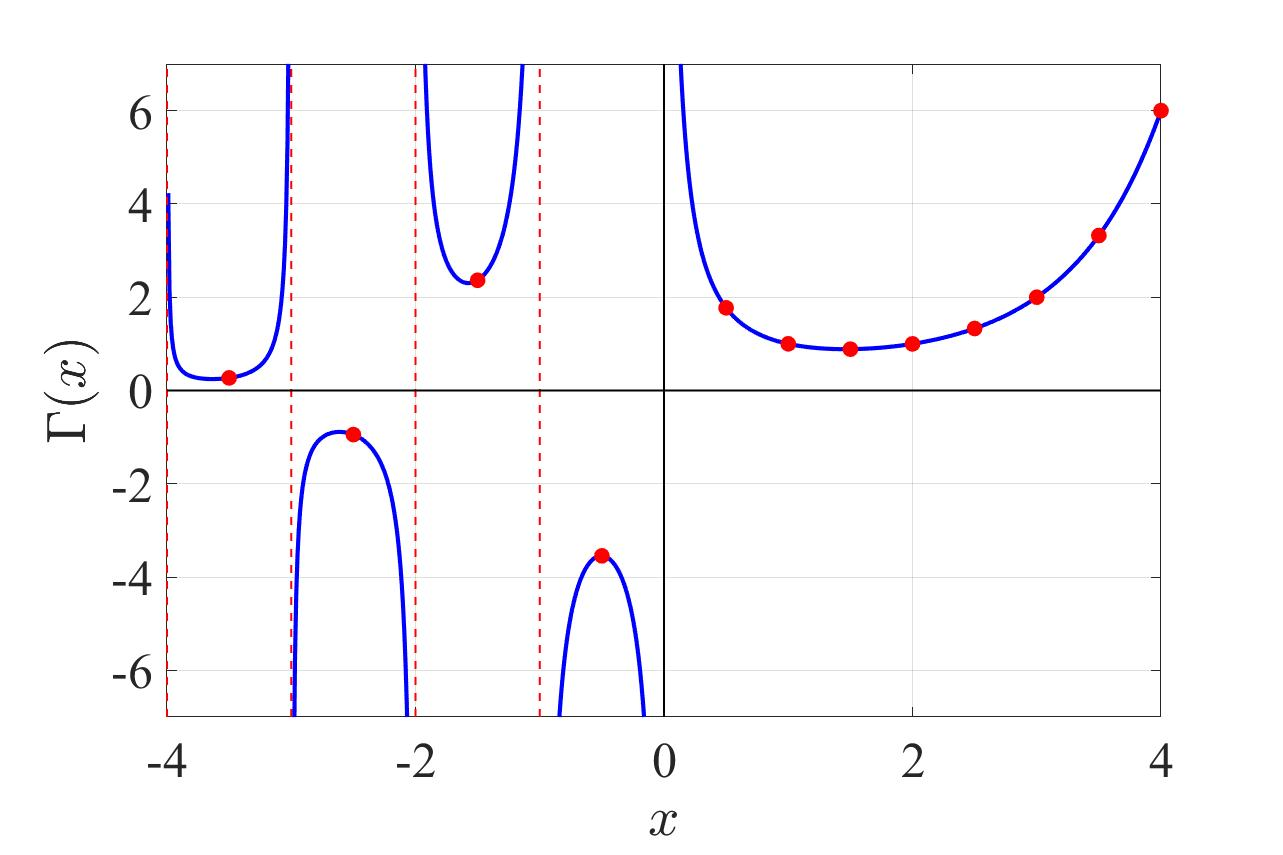
\includegraphics[width=1\textwidth]{matlab/gamma.jpg}
	\caption{函数$\Gamma\left(x\right)$的图像,其中$-4\le x \le 4$\label{fig:gammafig}}
\end{figure}

\begin{figure}[ht]
	\centering
	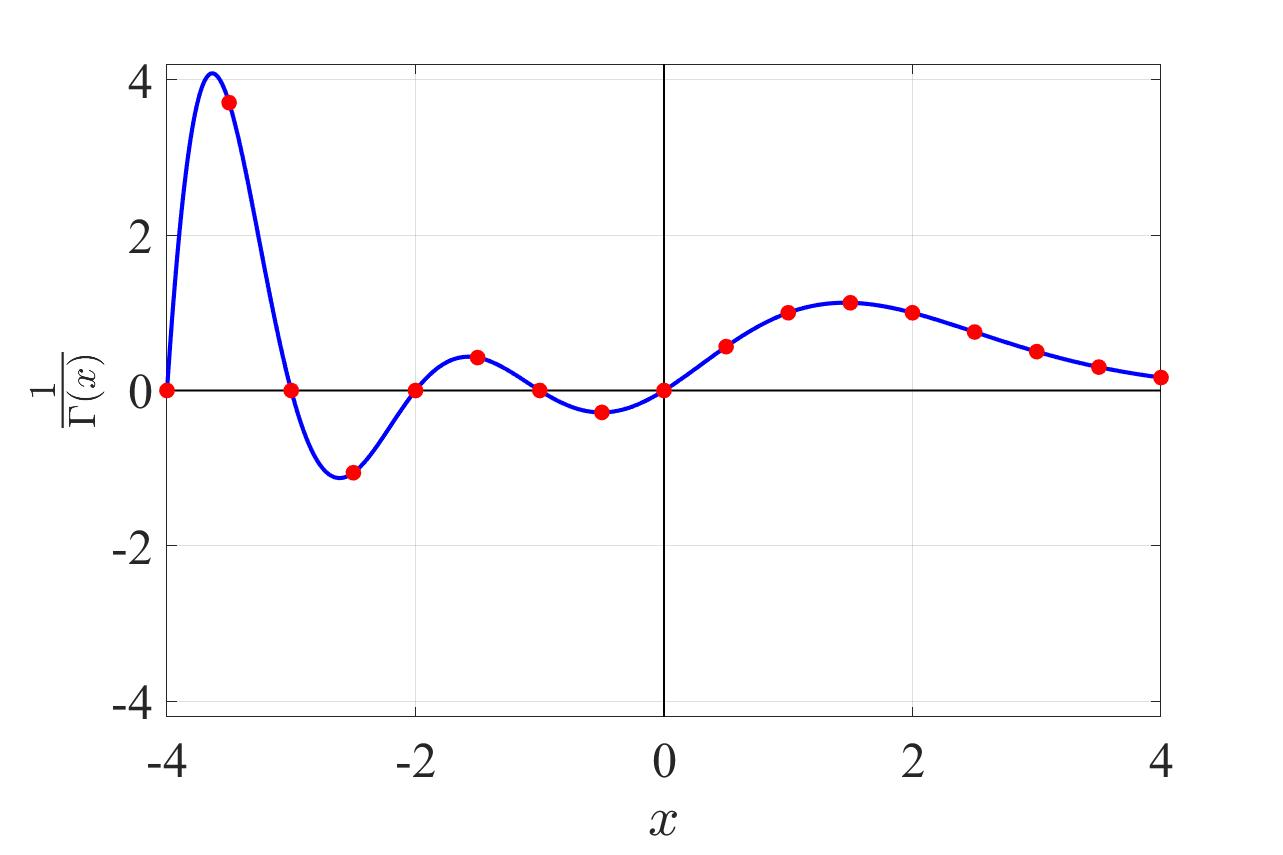
\includegraphics[width=1\textwidth]{matlab/invgamma.jpg}
	\caption{函数$\frac{1}{\Gamma\left(x\right)}$的图像,其中$-4\le x \le 4$\label{fig:invgammafig}}
\end{figure}

\begin{theorem}{Gamma函数收敛条件}
	当$\mathrm{Re}\left(z\right)>0$时Gamma函数收敛。
\end{theorem}

\begin{proof}
	此积分可以改写成
	$$ 	\Gamma\left(z\right) = \int_{0}^{\text{+}\infty }{x^{z-1}e^{-x}\mathrm{d}x}= \int_{0}^{1}{x^{z-1}e^{-x}\mathrm{d}x}+ \int_{1}^{\text{+}\infty }{x^{z-1}e^{-x}\mathrm{d}x}= I_1+I_2$$
	由于$e^{-x}$区间$[0,1]$有界且恒为正数,则$0<e^{-x}<e^0 = 1$,因此有
	$$\int_{0}^{1}{x^{z-1}e^{-x}\mathrm{d}x} < \int_{0}^{1}{x^{z-1}\mathrm{d}x} = \frac{1}{z}$$
	因此$I_1$ 显然收敛。
	由于
	$$1\le x \Rightarrow \frac{x^{z-1}}{e^{x/2}}\le 1 \Leftrightarrow x^{z-1}\le e^{x/2} \Leftrightarrow x^{p-1}e^{-x}\le e^{-x/2}$$
	因此有
	$$I_2 = \int_{1}^{\text{+}\infty }{x^{z-1}e^{-x}\mathrm{d}x}\le \int_{1}^{\text{+}\infty }{e^{-x/2}\mathrm{d}x} = 2e^{-1/2}$$
	因此$I_2$ 也是收敛的。
	
	此外当$\mathrm{Re}\left(z\right)\le 0$,积分$I_1$ 显然不收敛。因此得证当$\mathrm{Re}\left(z\right)>0$此积分收敛,当$\mathrm{Re}\left(z\right)\le0$此积分发散。	
\end{proof}


\begin{property}
	Gamma函数具有以下的性质:
	\begin{enumerate}[noitemsep]
		
		\item $\Gamma\left(x\right)$在区间$\left(0,+\infty\right)$连续的。但是$\displaystyle \frac{1}{\Gamma\left(x\right)}$在$\left(-\infty,+\infty\right)$上是连续的。
		
		\item $\Gamma\left(z+1\right) = z\Gamma\left(z\right).$
		\begin{proof}
			根据定义利用分布积分,有
			\begin{alignat*}{2}
			\Gamma\left(z+1\right) & = \int_{0}^{+\infty }{x^{z}e^{-x}\mathrm{d}x} \\
			& = \int_{0}^{+\infty }{-x^{z}\mathrm{d}e^{-x}} \\
			& = -x^{z}e^{-x}|_{0}^{+\infty} + \int_{0}^{+\infty}\left(z\right)x^{z-2}e^{-x}\mathrm{d}x
			& = 0 +z\int_{0}^{+\infty}x^{z-1}e^{-x}\mathrm{d}x \\
			& = z\Gamma\left(z\right)
			\end{alignat*}
			因此,得到$\Gamma\left(z+1\right) = z\Gamma\left(z\right).$
		\end{proof}
		
		\item 显然$\Gamma\left(1\right)=0!$,且对于任意正整数$n$,有$\Gamma\left(n\right)= \left(n-1\right)!$和$\Gamma\left(n+1\right)= n!$。 
		
		\item 对于任意正整数$n$,有
		$$\Gamma\left(z+n\right) = \left(z\right)_n\Gamma\left(z\right)$$
		通常的$\Gamma\left(z\right)$的计算方法是利用上述公式将其变换到区间$\left(0,1\right]$。若 $n<\mathrm{Re}\left(z\right)<n+1$,这里$n$为整数,即$n=\left[z \right]$,则
		$$
		\Gamma\left(z\right) = \Gamma\left(z-n\right) \times \left(z-n\right)_n = \Gamma\left(z-n\right) \times [\left(z-1\right)\left(z-2\right)...\left(z-n\right)]
		$$
		\item 由于当$z=0$第二类Euler积分发散,因此$\Gamma\left(0\right)=+\infty$。此外
		$$\Gamma\left(-n\right) = \frac{\Gamma\left(1-n\right)}{-n}= \frac{\Gamma\left(2-n\right)}{-n\left(1-n\right)} = \frac{\Gamma\left(3-n\right)}{-n\left(1-n\right)\left(2-n\right)} = \cdots = \left(-1\right)^n\frac{\Gamma\left(0\right)}{n!}= \left(-1\right)^n\frac{+\infty}{n!}$$
		
		\item 由于$\displaystyle \Gamma\left(z\right)=\frac{\Gamma\left(z+1\right)}{z}$,因此可以将Gamma函数可以推广的负数范围,即$-1<z<0$。根据此迭代关系,若$-n<z<1-n$,则
		$$\Gamma\left(z\right) = \frac{\Gamma\left(z+n\right)}{z\left(z+1\right)\left(z+2\right)\cdots\left(z+n-1\right)}=\frac{\Gamma\left(z+n\right)}{\left(z\right)_n}$$
		若$0<z<1$可将其写成
		\begin{alignat*}{2}
		\Gamma\left(z-n\right) & = \frac{\Gamma\left(z\right)}{\left(z-1\right)\left(z-2\right)\cdots\left(z-n\right)} = \frac{\Gamma\left(z\right)}{\left(z-n\right)_n}\\
		& \frac{\left(-1\right)^n\Gamma\left(z\right)}{\left(1-z\right)\left(2-z\right)\cdots\left(n-z\right)}= \frac{\left(-1\right)^n}{\left(1-z\right)_n}\Gamma\left(z\right)
		\end{alignat*}
		
		\item 当 $\displaystyle z = n+\frac{1}{2}$,其逆推关系为
		\begin{alignat*}{2}
		\Gamma \left(n+\frac{1}{2} \right) & = \left(n-\frac{1}{2}\right)\Gamma\left(n-\frac{1}{2}\right) = \left(n-\frac{1}{2}\right)\left(n-\frac{3}{2}\right)\Gamma\left(n-\frac{3}{2}\right) = \left(n-\frac{1}{2}\right)\left(n-\frac{3}{2}\right)\cdots \frac{5}{2}\frac{3}{2}\frac{1}{2}\Gamma \left(\frac{1}{2} \right)\\
		& = \frac{\left(2n-1\right)!!}{2^n}\Gamma\left(\frac{1}{2}\right) = \frac{\left(2n\right)!}{n!2^{2m}}\Gamma\left(\frac{1}{2}\right)
		\end{alignat*}
		
		\item $\Gamma\left(z\right)$也可以通过下列方式定义
		\begin{equation}\label{eq:gammalog}
		\Gamma\left(z\right) = \int_{0}^{1}\left[\ln \left(\frac{1}{y} \right) \right]^{p-1}dy
		\end{equation}
		\begin{proof}	
			利用$y = e^{-x}$此积分可以改写成
			$$\int_{0}^{1}\left[\ln \left(\frac{1}{y} \right) \right]^{p-1}dy = \int_{+\infty}^{0}-x^{p-1}e^{-x}dx =  \int_{0}^{+\infty}x^{p-1}e^{-x}dx = \Gamma\left(x\right)$$
			因此 $\Gamma\left(z\right)$也可以使用式~\ref{eq:gammalog}进行定义。
		\end{proof}	
		
		\item $ \displaystyle \Gamma \left(\frac{1}{2} \right)= \sqrt{\pi}.$
		\begin{proof}
			根据定义利用Gamma函数的定义,有
			$$\Gamma  \left(\frac{1}{2} \right) = \int_{0}^{\text{+}\infty }{x^{-\frac{1}{2}}e^{-x}\mathrm{d}x} $$令$\displaystyle x = \frac{u^2}{2}$,则 $ \displaystyle x^{-\frac{1}{2}} = \frac{\sqrt{2}}{u}$,$dx = udu$,代入上式得到
			$$ \Gamma  \left(\frac{1}{2} \right) = \int_{0}^{\text{+}\infty }\frac{\sqrt{2}}{u} e^{-\frac{u^2}{2}} u\mathrm{d}u = \frac{1}{2}\int_{-\infty}^{+\infty }\frac{\sqrt{2} \sqrt{2\pi}}{\sqrt{2\pi}} e^{-\frac{u^2}{2}} \mathrm{d}u = \sqrt{\pi} \int_{-\infty}^{+\infty }\frac{1}{\sqrt{2\pi}} e^{-\frac{u^2}{2}} u\mathrm{d}u$$
			根据正态分布可知$\displaystyle \int_{-\infty}^{+\infty }\frac{1}{\sqrt{2\pi}} e^{-\frac{u^2}{2}} \mathrm{d}u = 1$,由于
			$$ I = \int_{-\infty}^{+\infty }\frac{1}{\sqrt{2\pi}} e^{-\frac{u^2}{2}} \mathrm{d}u = \int_{-\infty}^{+\infty }\frac{1}{\sqrt{2\pi}} e^{-\frac{v^2}{2}} \mathrm{d}v$$
			则二重积分
			$$ I^2 = \int_{-\infty}^{+\infty }\frac{1}{\sqrt{2\pi}} e^{-\frac{u^2}{2}} \mathrm{d}u \int_{-\infty}^{+\infty }\frac{1}{\sqrt{2\pi}} e^{-\frac{v^2}{2}} \mathrm{d}v = \int_{-\infty}^{+\infty } \int_{-\infty}^{+\infty } \frac{1}{2\pi}  e^{-\frac{u^2+v^2}{2}}\mathrm{d}u \mathrm{d}v$$
			令$u = r\cos\left(\theta\right),v = r\sin\left(\theta\right)$,则 $0\le r<+\infty,0\le \theta <2\pi$ 和  $\mathrm{d}x\mathrm{d}y = r\mathrm{d}r\mathrm{d}\theta $,代入上式得到
			则二重积分可以转化为
			$$ I^2 = \int_{0}^{2\pi}\int_{0}^{+\infty } \frac{1}{2\pi}  re^{-r^2}\mathrm{d}r \mathrm{d}\theta = 1.$$
			由于 $I >0$,因此得到$ I = 1$.
			因此$\displaystyle \Gamma\left(\frac{1}{2}\right) = \sqrt{\pi}$。
			此式也可以利用反射性质(后文会给出证明)进行证明,由于
			$$\Gamma\left(p\right)\Gamma\left(1-p\right) = \frac{\pi}{\sin\left(\pi p\right)},\quad 0<p<1.$$
			令 $\displaystyle p = \frac{1}{2}$,得到 $\displaystyle \Gamma\left(\frac{1}{2}\right)\Gamma\left(\frac{1}{2}\right) = \frac{\pi}{1} = \pi$
			因此也可以证明得到$\displaystyle \Gamma\left(\frac{1}{2}\right) = \sqrt{\pi}$。
		\end{proof}
		
		\item 常用非整数的Gamma函数的值如下:
		\begin{alignat*}{2}
		&\Gamma\left(-\frac{1}{2}\right) = -2\sqrt{\pi},\quad  \Gamma\left(\frac{3}{2}\right) = \frac{1}{2}\sqrt{\pi},\quad  \Gamma\left(\frac{5}{2}\right) = \frac{3}{4}\sqrt{\pi},\\
		& \Gamma\left(\frac{1}{3}\right) = 2.678938,\quad \Gamma\left(n+\frac{1}{3}\right) = \frac{1\times 4 \dots \left(3n-2\right)}{3^n}\Gamma\left(\frac{1}{3}\right),\\
		&\Gamma\left(\frac{2}{3}\right) = 1.354118,\quad \Gamma\left(n+\frac{2}{3}\right) = \frac{2\times 5 \dots \left(3n-1\right)}{3^n}\Gamma\left(\frac{2}{3}\right),\\
		&\Gamma\left(\frac{1}{4}\right) = 3.625600,\quad \Gamma\left(n+\frac{1}{4}\right) = \frac{1\times 5 \dots \left(4n-3\right)}{4^n}\Gamma\left(\frac{1}{4}\right),\\
		&\Gamma\left(\frac{3}{4}\right) = 1.225417,\quad \Gamma\left(n+\frac{3}{4}\right) = \frac{3\times 7 \dots \left(4n-1\right)}{4^n}\Gamma\left(\frac{3}{4}\right).\\
		\end{alignat*}
		
		\item Gamma函数与组合数和排列数的关系:
		\begin{alignat*}{2}
		&\Gamma\left(p+1\right) = p! = A^1_p = A\left(p,1\right) = P^1_p = P\left(p,1\right), \quad p \in \mathbb{N},\\
		&\frac{\Gamma\left(p+1\right)}{\Gamma\left(q+1\right)}  = \frac{p!}{q!}= A^q_p = P^q_p = A\left(p,q\right) = P\left(p,q\right), \quad p,q \in \mathbb{N},q \le p,\\
		& \frac{\Gamma\left(p+1\right)}{\Gamma\left(q+1\right)\Gamma\left(p-q+1\right)} = \binom{p}{q} = C_p^q = C(p,q)=C(p,{p-q}) , \quad p,q \in \mathbb{N},q \le p.
		\end{alignat*}
		
		
		
		\item 此外Gamma函数有其他几种定义的方式,即:
		\begin{enumerate}[noitemsep]
			
			\item Euler无穷乘积(Gauss形式)
			\begin{equation}
			\Gamma\left(z\right)=\frac{1}{z}\prod _{k=1}^{+\infty}{\frac {\left(1+\frac{1}{k}\right)^{z}}{1+{\frac{z}{k}}}},\quad \mathrm{Re}\left(z\right) \ne  0,-1,-2,\cdots.
			\end{equation}
			\begin{equation}
			\Gamma\left(z\right) = \lim_{n \to {\infty}} n! \; n^z\prod_{k=0}^{n}{\frac{1}{z+k}},\quad \mathrm{Re}(z) \ne 0,-1,-2,\cdots
			\end{equation}
			\begin{proof}	
				根据极限的知识$e^{-x}$
				可以表达为$$e^{-x}=\lim _{k \rightarrow +\infty}\left(1-\frac{x}{k}\right)^{k}.$$		
				因此可以得到$$\Gamma\left(z\right) = \int_{0}^{\infty} e^{-x} x^{p-1} \mathrm{d} x=\lim _{k \rightarrow +\infty} \int_{0}^{k}\left(1-\frac{x}{k}\right)^{k} x^{z-1}  \mathrm{d}  x$$
				令$x = tk$,因此$\mathrm{d}x = l\mathrm{d}t $,代入上式有
				$$\Gamma\left(z\right) = \int_{0}^{\infty} e^{-kt} x^{p-1} \mathrm{d} x=\lim _{k \rightarrow \infty} \int_{0}^{1}\left(1-t\right)^{k} (kt)^{z-1} k\mathrm{d} t = \lim _{k \rightarrow \infty} k^z \int_{0}^{1}\left(1-t\right)^{k} t^{z-1}  \mathrm{d} t$$
				对于积分使用分部积分法则,即
				\begin{alignat*}{2}
				\int_{0}^{1}\left(1-t\right)^{k} t^{z-1} \mathrm{d} t & = \frac{1}{z} \int_{0}^{1}\left(1-t\right)^{k} \mathrm{d} t^z =  \frac{1}{z} \left(1-t\right)^{k} t^z \Big| ^1_0 + \frac{k}{z} \int_{0}^{1}\left(1-t\right)^{k-1}t^z \mathrm{d} t\\
				& = \frac{k}{z} \int_{0}^{1}\left(1-t\right)^{k-1}t^z \mathrm{d} t
				\end{alignat*}
				重复上述过程有
				$$\Gamma\left(z\right) = \lim _{k \rightarrow +\infty} {\frac{k^z k!}{z(z+1)\cdots(z+k)}}.$$
				由于
				$$
				\lim _{k \rightarrow +\infty} \frac{\left(k+1\right)^z}{k^z} = \lim _{k \rightarrow +\infty}{\left(\frac{k+1}{k}\right)^z} = \lim _{k \rightarrow +\infty}{\left(1+\frac{1}{k}\right)^z} = 1
				$$
				因此可以得到
				$$\Gamma\left(z\right) = \lim _{k \rightarrow +\infty} {\frac{\left(k+1\right)^z k!}{z\left(z+1\right)\cdots\left(z+k \right)}} = \frac{1}{z}\lim _{k \rightarrow +\infty}{\frac{1}{\left(1+z \right)\left(1+\frac{z}{2}\right)\cdots \left(1+\frac{z}{k}\right)}} \frac{2^z3^z\cdots \left(k+1\right)^z}{1^z2^z\cdots k^z}.$$
				可以表示为
				$$\Gamma\left(z\right) = \frac{ 1}{z} \prod_{k = 1}^{+\infty}\frac{1}{1+\frac{z}{k}}\frac{\left(k+1\right)^p}{k^p} = \frac{1}{z} \prod_{k = 1}^{+\infty}\left(1+\frac{z}{k}\right)^{-1}\left(1+\frac{1}{k}\right)^p,\quad \mathrm{Re}(z) \ne 0,-1,-2,\cdots $$
			\end{proof}	
			
			\item Weierstrass形式
			\begin{equation}
			\Gamma \left(z\right)={\frac {e^{-\gamma z}}{z}}\prod _{k=1}^{\infty }{\left(1+{\frac {z}{k}}\right)^{-1}e^{z/k}},\quad \mathrm{Re}(z) \ne 0,-1,-2,\cdots
			\end{equation}
			其中$\gamma $为欧拉常数 \cite{Wiki-Euler-Mascheroni-constant} ,其表达式为
			$$ \gamma =  \lim _{n \rightarrow +\infty} {\left[\sum_{k=1}^n {\frac{1}{k}} \right]-\ln \left(n\right)}  = \int _{1}^{+\infty }\left(-{\frac {1}{x}}+{\frac {1}{\lfloor x\rfloor }}\right)\mathrm{d}x \approx 0.577215663\dots$$
			这里$\lfloor x\rfloor$表示不大于$x$的最大整数。
			\begin{proof}
				Gauss形式的$\Gamma\left(z\right)$可以表示为
				$$\Gamma\left(z\right) = \lim _{k \rightarrow +\infty} {\frac{k^z k!}{z\left(z+1\right)\cdots\left(z+k \right)}},\quad \mathrm{Re}(z) \ne 0,-1,-2,\cdots$$		 		
				这里$k^z$可以表示为$$
				k^z = e^{z\ln \left(k\right)} =e^{p\left[\ln\left(k\right)-1-\frac{1}{2}-\cdots-\frac{1}{k}\right]}e^{z \left(1+\frac{1}{2}+\cdots+\frac{1}{k} \right)}
				$$
				$$
				\Gamma_k\left(z\right) = \frac{k^z k!}{z\left(z+1\right)\cdots\left(z+k \right)} = \frac{e^{z\left[\ln\left(k\right)-1-\frac{1}{2}-\cdots-\frac{1}{k}\right]}e^{z \left(1+\frac{1}{2}+\cdots+\frac{1}{k}\right)}}{z\left(1+z \right)\left(1+\frac{z}{2}\right)\cdots \left(1+\frac{z}{k}\right)}
				$$
				因此$$
				\Gamma\left(z\right) = \lim _{k \rightarrow +\infty}\Gamma_k\left(z\right) = e^{-\gamma z} \lim _{k \rightarrow +\infty}\frac{e^z}{1+z} \frac{e^{\frac{z}{2}}}{1+\frac{z}{2}}\cdots \frac{e^{\frac{z}{k}}}{1+\frac{z}{k}} =  \frac{e^{-\gamma z}}{z}  \prod_{k=1}^{+\infty}\frac{e^{\frac{z}{k}}}{1+\frac{z}{k}} = e^{-\gamma z}  \prod_{k=0}^{+\infty}\frac{e^{\frac{z}{k}}}{1+\frac{z}{k}}   $$
				或可以写成$$\frac{1}{\Gamma\left(z\right)} =  ze^{\gamma z}\prod_{k=1}^{+\infty}\left(1+\frac{z}{k}\right)e^{-\frac{z}{k}} =e^{\gamma z}\prod_{k=0}^{+\infty}\left(1+\frac{z}{k}\right)e^{-\frac{z}{k}}$$	
			\end{proof}
			
			\item 广义Laguerre多项式\cite{Wiki-Laguerre-Polynomials}形式 
			\begin{equation}
			\Gamma \left(z,x\right)=x^{z}e^{-x}\sum _{n=0}^{\infty }{\frac {L_{n}^{\left(z\right)}\left(x\right)}{n+1}},\quad \mathrm{Re}\left(z\right)>-1,\quad x>0.
			\end{equation}
			\begin{equation}
			\Gamma \left(z\right)=t^{z}\sum _{n=0}^{\infty }{\frac {L_{n}^{\left(z\right)}\left(t\right)}{z+n}},\quad \mathrm{Re}\left(z\right)<\frac{1}{2}
			\end{equation}
			\begin{proof}
				\hint{待补充} \url{https://dlmf.nist.gov/8.7}
			\end{proof}
		\end{enumerate}
		
		\item Gamma函数的反射性质为
		\begin{equation}
		\Gamma\left(z\right)\Gamma\left(1-z\right) = \frac{\pi}{\sin\left(\pi z\right)},\quad 0<p<1.
		\end{equation}
		
		\begin{proof}
			根据Gamma函数的Weierstrass形式有
			\begin{alignat*}{2}
			\Gamma\left(z\right)\Gamma\left(-z\right) & = \frac{e^{-\gamma z}}{z} \prod_{k=1}^{+\infty}\frac{e^{\frac{z}{k}}}{1+\frac{z}{k}}\frac{e^{\gamma z}}{-z} \prod_{k=1}^{+\infty}\frac{e^{-\frac{z}{k}}}{1-\frac{z}{k}} \\ 
			& = -\frac{1}{z^2}\prod_{k=1}^{+\infty}\frac{k^2}{k^2-z^2}
			\end{alignat*}
			由于$\displaystyle \Gamma(-z)= -\frac{\Gamma(1-z)}{z}$,则
			$$\Gamma\left(z\right)\Gamma\left(1-z\right) = - z \Gamma\left(z\right)\Gamma\left(-z\right) = \frac{1}{z}\prod_{k=1}^{+\infty}\frac{k^2}{k^2-z^2},$$
			$$\frac{1}{\Gamma\left(z\right)\Gamma\left(1-z\right)} = z\prod_{k=1}^{+\infty}\left(1-\frac{z^2}{k^2}\right).$$
			\hint{待补充 } \url{https://en.wikipedia.org/wiki/Sine}
			
			由于$\sin(\pi z)$可以表示为
			$$\sin(\pi z)=\pi z\prod _{n=1}^{\infty }\left(1-{\frac {z^{2}}{n^{2}}}\right).$$
			因此得证
			$$\Gamma\left(z\right)\Gamma\left(1-z\right) = \frac{\pi}{\sin\left(\pi z\right)}.$$
			也可以按照下列步骤进行证明,由于
			\begin{alignat*}{2}
			\Gamma\left(z\right) \Gamma\left(1-z\right) & = \int_0^{+\infty} e^{-t} t^{z-1} \mathrm{d}t \int_0^{+\infty} e^{-s} s^{1-z-1} \mathrm{d}s \\
			& = \int_0^{+\infty} \int_0^{+\infty} e^{-\left(s+t\right)} \left(\frac{t}{s}\right)^z t^{-1} \mathrm{d}s \mathrm{d}t               
			\end{alignat*}
			做积分变换$$t+s=u,\frac{t}{s}=v,t = \frac{uv}{1+v},s = \frac{u}{1+v}$$
			因此Jacobian矩阵的行列式为
			$$
			\frac{D\left[s,t\right]}{D\left[u,v\right]} = \begin{Vmatrix}
			\frac{v}{v+1}& \frac{u}{v+1} \\ -\frac{1}{v+1}& \ - \frac{u}{v+1}
			\end{Vmatrix} = -\frac{v}{\left(v+1\right)^2}
			$$
			因此原积分为
			$$\Gamma\left(z\right) \Gamma\left(1-z\right) = \int_0^{1} -\frac{v^{z-1}}{1+v} \mathrm{d}v =  \int_0^{1} \frac{v^{z}}{1+v} \mathrm{d}v =  \frac{\pi}{\sin\left(\pi z\right)}. $$
			\hint{待补充 复变函数} 
		\end{proof}
		
	\end{enumerate}
\end{property}



\subsection{Beta函数}
在多数情况下,使用Beta函数\cite{Wiki-Beta-Function}的某些组合比Gamma函数更方便。Beta函数通常定义为以下形式。

\begin{definition}{Beta函数}{Beta Function}
	第一类Euler积分
	$$ \mathrm{B}\left(z,\omega\right) = \int_{0}^{1}{x^{z-1}\left(1-x\right)^{\omega-1}\mathrm{d}x},\quad  \mathrm{Re}\left(z\right)>0, \quad \mathrm{Re}\left(\omega\right)>0,$$
	称为Beta函数,且$$\mathrm{B}\left(z,1\right) = \mathrm{B}\left(1,z\right) = \frac{1}{z}.$$
\end{definition}

\begin{property}
	Beta函数具有以下的一些基本性质:
	\begin{enumerate}[noitemsep]
		
		\item 若$\mathrm{Re}\left(\omega\right)>0,\mathrm{Re}\left(z\right)>0$,则有交换性质(Symmetric)
		\begin{equation}
		\mathrm{B}\left(z,\omega\right)= \mathrm{B}\left(\omega,z\right).
		\end{equation}
		\begin{proof}
			利用积分变换 $y = 1-x$,有
			$$\int_{0}^{1}{x^{z-1}\left(1-x\right)^{\omega-1}\mathrm{d}x} = \int_{1}^{0}{-\left(1-y\right)^{z-1}y^{\omega-1}\mathrm{d}y} = \int_{0}^{1}{y^{\omega-1}\left(1-y\right)^{z-1}\mathrm{d}y},$$
			因此有$$\mathrm{B}\left(z,\omega\right)= \mathrm{B}\left(\omega,z\right).$$
		\end{proof}
		\item 若$\mathrm{Re}\left(\omega\right)>0,\mathrm{Re}\left(z\right)>1$,则
		\begin{equation}
		\mathrm{B}\left(\omega,z\right)=  \frac{z-1}{\omega+z-1}\mathrm{B}\left(\omega,z-1\right).
		\end{equation}
		\begin{proof}
			\begin{alignat*}{2}
			\mathrm{B}\left(\omega,z\right) & = \int_{0}^{1}{x^{z-1}\left(1-x\right)^{\omega-1}\mathrm{d}x}\\
			& = \int_{0}^{1}\frac{1}{z}\left(1-x\right)^{\omega-1}\mathrm{d}x^z \\
			& = \frac{1}{z}\left(1-x\right)^{\omega-1}x^z\Big|^1_0 + \frac{\omega-1}{z} \int_{0}^{1}\left(1-x\right)^{\omega-2}x^z \mathrm{d}x \\
			& =  \frac{\omega-1}{z} \int_{0}^{1}\left(1-x\right)^{\omega-2}x^{z-1} - \left(1-x\right)^{\omega-1}x^{z-1}\mathrm{d}x \\
			& = \frac{\omega-1}{z} \int_{0}^{1}{x^{z-1}\left(1-x\right)^{\omega-2}\mathrm{d}x}-\frac{\omega-1}{z}\int_{0}^{1}{x^{z-1}\left(1-x\right)^{\omega-1}\mathrm{d}x} \\
			& = \frac{\omega-1}{z}\mathrm{B}\left(z,\omega-1\right)-\frac{\omega-1}{z}\mathrm{B}\left(z,\omega\right) 
			\end{alignat*}
			因此$$\mathrm{B}\left(\omega,z\right)=  \frac{z-1}{\omega+z-1}\mathrm{B}\left(\omega,z-1\right).$$
		\end{proof}
		利用上面的结论可以证明下面的三个性质:
		\begin{enumerate}[noitemsep]
			\item $\displaystyle \mathrm{B}\left(x,y\right) =  \mathrm{B}\left(x,y+1\right)+ \mathrm{B}\left(x+1,y\right)$
			\item $\displaystyle \mathrm{B}\left(x+1,y\right) = \mathrm{B}\left(x,y\right)\cdot \frac{x}{x+y}.$
			\item $\displaystyle \mathrm{B}\left(x,y+1\right) = \mathrm{B}\left(x,y\right)\cdot \frac{y}{x+y}.$
		\end{enumerate}
		\begin{proof}
			直接利用上述性质,便可以证明(2)和(3)式,(2)和(3)式相加,可以证明(1)式。
		\end{proof}
		\item Beta函数与Gamma函数有如下的关系式:
		\begin{equation}
		\mathrm{B}\left(z,\omega\right) = \frac{\Gamma\left(z\right) \Gamma\left(\omega\right)}{\Gamma\left(z+\omega\right)}.
		\end{equation}
		\begin{proof}
			即证明:
			$$\mathrm{B}\left(x,y\right)=\frac{\Gamma\left(x\right)\Gamma\left(y\right)}{\Gamma\left(x+y\right)}.$$
			其中 $$\Gamma\left(x\right)=\int_0^{+\infty} e^{-t} t^{x-1} \mathrm{d}t,\quad \mathrm{B} \left(x,y\right)=\int_0^1 t^{x-1}\left(1-t\right)^{y-1} \mathrm{d}t.$$
			则$\Gamma\left(x\right) \Gamma\left(y\right)$可表示
			$$\Gamma\left(x\right) \Gamma\left(y\right)  = \int_0^{+\infty} e^{-t} t^{x-1} \mathrm{d}t \int_0^{+\infty} e^{-s} s^{y-1} \mathrm{d}s = \int_0^{+\infty} \int_0^{+\infty} e^{-\left(s+t\right)} t^{x-1} s^{y-1} \mathrm{d}s \mathrm{d}t.$$
			作积分变换 $t=u^2,s=v^2$,则
			$$
			\Gamma\left(x\right) \Gamma\left(y\right) = 4 \int_0^{+\infty} \int_0^{+\infty} e^{-\left(u^2+v^2\right)} u^{2x-2} v^{2y-2} uv \mathrm{d}u \mathrm{d}v = 4 \int_0^{+\infty} \int_0^{+\infty} e^{-\left(u^2+v^2\right)} u^{2x-1} v^{2y-1} \mathrm{d}u  \mathrm{d}v.
			$$			
			作积分变换 $u=r\cos \theta,v=r\sin \theta$,则
			$$
			\Gamma\left(x\right) \Gamma\left(y\right) = 2 \int_0^{+\infty} r e^{-r^2} r^{2x+2y-2} \mathrm{d}r 2\int_0^{\frac{\pi}{2}} |\cos \theta|^{2x-1} |\sin \theta|^{2y-1} \mathrm{d} \theta.
			$$
			其前部分作积分变换$s = r^2$,则
			$$ 2 \int_0^{+\infty} r e^{-r^2} r^{2x+2y-2} \mathrm{d}r = \int_0^{+\infty} e^{-s} s^{x+y-1} \mathrm{d}s =  \Gamma\left(x+y\right).$$
			其中后半部分作积分变换$t=\cos^2 \theta$,则
			$$2 \int_0^{\frac{\pi}{2}} |\cos \theta|^{2x-1} |\sin \theta|^{2y-1} \mathrm{d} \theta = 2 \int_0^{1} t^{x-\frac{1}{2}} \left(1-t\right)^{y-\frac{1}{2}} \frac{1}{2} t^{-\frac{1}{2}}  \left(1-t\right)^{-\frac{1}{2}} \mathrm{d}t = \int_0^1 t^{x-1} \left(1-t\right)^{y-1} \mathrm{d}t = \mathrm{B} \left(x,y\right).
			$$
			故得证上式
			$$\mathrm{B}\left(x,y\right)=\frac{\Gamma\left(x\right)\Gamma\left(y\right)}{\Gamma\left(x+y\right)}. $$
		\end{proof}
		\item 从上述过程可以得到Beta函数其他定义表达式:
		\begin{enumerate}[noitemsep]
		\item $	\displaystyle {\mathrm{B}\left(x,y\right)}= \frac{\Gamma\left(x\right)\Gamma\left(y\right)}{\Gamma\left(x+y\right)},\quad \mathrm{Re}\left(x\right)>0,\mathrm{Re}\left(y\right)>0	.$
		
		\item $	\displaystyle  {\mathrm{B}\left(x,y\right)}= \frac{\left(x-1\right)!\left(y-1\right)!}{\left(x+y-1\right)!},\quad x,y \in \mathbb{N^*}.$
		
		\item $ \displaystyle  {\mathrm{B}\left(x,y\right)}= 2\int_0^{\frac{\pi}{2}} |\cos \theta|^{2x-1} |\sin \theta|^{2y-1} \mathrm{d} \theta,\quad \mathrm{Re}\left(x\right)>0,\mathrm{Re}\left(y\right)>0	.$
		
		\item 	$\displaystyle  {\mathrm{B}\left(x,y\right)}=  \int _{0}^{\infty }{\frac {t^{x-1}}{(1+t)^{x+y}}}\mathrm{d} t,\quad \mathrm{Re}\left(x\right)>0,\mathrm{Re}\left(y\right)>0.	$
		
		\item $\displaystyle 	{\mathrm{B}\left(x,y\right)}=  n\int _{0}^{1}t^{nx-1}(1-t^{n})^{y-1}\mathrm{d} t,\quad \mathrm{Re}\left(x\right)>0,\mathrm{Re}\left(y\right)>0,n>0.	$
		
		\item $\displaystyle {\mathrm{B}\left(x,y\right)}=  \sum _{n=0}^{\infty }{\frac {C^n_{n-y}}{x+n}},\quad \mathrm{Re}\left(x\right)>0,\mathrm{Re}\left(y\right)>0.
		$
		
		\item $\displaystyle \mathrm {B} (x,y)={\frac {x+y}{xy}}\prod _{n=1}^{\infty }\left(1+{\dfrac {xy}{n(x+y+n)}}\right)^{-1},\quad \mathrm{Re}\left(x\right)>0,\mathrm{Re}\left(y\right)>0.$
		
		\end{enumerate}
		
		\item Beta函数与组合数的关系:若 $ m,n \in \mathbb{N^*}$,则
		\begin{alignat*}{2}
		{\mathrm{B}\left(m,n\right) }&= \mathrm{B}\left(n,m\right) = \frac{\Gamma\left(m\right)\Gamma\left(n\right)}{\Gamma\left(m+n\right)}= \frac{1\cdot2 \cdot 3 \dots \left(n-1\right)}{m\cdot \left(m+1\right) \cdot \left(m+2\right) \dots \left(m+n-1\right)} \\
		& =\frac{\left(n-1\right)!\left(m-1\right)!}{\left(n+m-1\right)!} = \frac{1}{\left(n+m-1\right)C^{n-1}_{n+m-2}} = \frac{1}{\left(n+m-1\right)C^{m-1}_{n+m-2}}
		\end{alignat*}
		$$
		C^m_{m+n} = C^n_{m+n} = \frac{\left(m+n\right)!}{m!n!} = \frac{1}{\left(n+m+1\right)\mathrm{B}(m+1,n+1)} = \frac{1}{\left(n+m+1\right)\mathrm{B}(n+1,m+1)}
		$$
		$$
		C^m_n = \frac{1}{\left(n+1\right)\mathrm{B}(n-m+1,m+1)},\quad C^m_n = C^{n-m}_n = C^{m-1}_{n-1} +  C^{m}_{n-1},\quad C^m_n = \frac{m}{n}C^{m-1}_{n-1}
		$$
		$$
		\quad \frac{1}{\left(n+1\right)\mathrm{B}(n-m+1,m+1)} = \frac{1}{n\mathrm{B}(n-m+1,m)}+\frac{1}{n\mathrm{B}(n-m,m+1)} 
		$$
		$$ \quad \frac{1}{\left(n+1\right)\mathrm{B}(n-m+1,m+1)} = \frac{m}{n^2\mathrm{B}(n-m+1,m)} 
		$$
		以上结果,将Beta函数展开成Gamma函数和排列组合数便可进行证明。
		\item 借助Beta函数,可以建立Gamma函数的三个重要的关系。
		\begin{enumerate}
			\item 第一个重要关系是
			\begin{equation}
			\Gamma \left(1-z\right)\Gamma\left(z\right) = {\mathrm{B}\left(z,1-z\right) } =\frac{\pi}{\sin {\left(\pi z\right)}}, \quad z\not \in \mathbb{Z}.
			\end{equation}
			\begin{equation}
			\Gamma \left(\varepsilon -n\right)=\left(-1\right)^{n-1}\;{\frac {\Gamma \left(-\varepsilon \right)\Gamma \left(1+\varepsilon \right)}{\Gamma \left(n+1-\varepsilon \right)}}.
			\end{equation}
			\begin{equation}
				\mathrm {B} (x,y) \cdot \mathrm {B} (x+y,1-y)={\frac {\pi }{x\sin(\pi y)}}.
			\end{equation}
			
			\begin{proof}
				由于
				$$\Gamma \left(1-z\right)\Gamma\left(z\right) = \mathrm{B}\left(1-z,z\right)\Gamma\left(1\right) = \int_{0}^{1}{x^{z-1}\left(1-x\right)^{-z}\mathrm{d}x}.$$
				由于\hint{待补充} \url{https://dlmf.nist.gov/5.12},因此得证第式(1)。
				$$\Gamma \left(1-z\right)\Gamma\left(z\right) = \int_{0}^{1}{x^{z-1}\left(1-x\right)^{-z}\mathrm{d}x} = \frac{\pi}{\sin {\left(\pi z\right)}}.$$
				而由于
				$$  \Gamma \left(\varepsilon -n\right) \Gamma \left(n+1-\varepsilon \right) = \frac{\pi}{\sin\left(\pi\left(\varepsilon-n\right)\right)} = \left(-1\right)^n\frac{\pi}{\sin\left(\pi \varepsilon\right)} $$
				$$
				\Gamma \left(-\varepsilon \right)\Gamma \left(1+\varepsilon \right) = \frac{\pi}{\sin\left(-\pi\varepsilon\right)} = -\frac{\pi}{\sin\left(\pi \varepsilon\right)}
				$$
				因此得证上式(2)。
				此外由于
				$$ \mathrm {B} (x,y) \cdot \mathrm {B} (x+y,1-y) = \frac{\Gamma\left(x\right)\Gamma\left(y\right)}{\Gamma\left(x+y\right)}\cdot \frac{\Gamma\left(x+y\right)\Gamma\left(1-y\right)}{\Gamma\left(x+1\right)} = \frac{\Gamma\left(y\right)\Gamma\left(1-y\right)}{x} = {\frac {\pi }{x\sin(\pi y)}}.
				$$
				因此得证上式(3)。
			\end{proof}
			
			\item 第二个重要的关系是Legendre公式:
			\begin{equation}
			\Gamma \left(z\right)\Gamma\left(z+\frac{1}{2}\right)=2^{1-2z}{\sqrt {\pi }}\Gamma\left(2z\right),\quad  2z \neq 0,-1,-2,\cdots.
			\end{equation}
			\begin{equation}
			 \Gamma\left(2z\right) = \frac{2^{2z-1}}{\sqrt {\pi }}\Gamma \left(z\right)\Gamma\left(z+\frac{1}{2}\right).
			\end{equation}			
			\begin{proof}
				令 $x = y = z$代入$ \mathrm {B} (x,y) $,则
				$$ \mathrm {B} (z,z) = \frac{\Gamma\left(z\right)\Gamma\left(z\right)}{\Gamma\left(2z\right)} = \int_{0}^{1}u^{z-1}\left(1-u\right)^{z-1}\mathrm{d}u$$ 
			令 $\displaystyle u= \frac{1+x}{2}$,则
			$$\frac{\Gamma^2\left(z\right)}{\Gamma\left(2z\right)} = \frac{1}{2^{2z-1}}\int_{-1}^{1}\left(1-x^2\right)^{z-1}\mathrm{d}x = \frac{1}{2^{2z-1}}\cdot 2 \int_{0}^{1}\left(1-x^2\right)^{z-1}\mathrm{d}x$$
			由于$\displaystyle \mathrm{B}\left(\frac{1}{2},z\right)$可以表示为
			$$\mathrm{B}\left(\frac{1}{2},z\right) = \int_{0}^{1}{t^{-\frac{1}{2}}\left(1-t\right)^{z-1}\mathrm{d}t}.$$
			做积分变换$t = x^2$
			$$\mathrm{B}\left(\frac{1}{2},z\right) = 2\int_{0}^{1}{\left(1-x^2\right)^{z-1}\mathrm{d}x}.$$
			因此	
			$$\frac{\Gamma^2\left(z\right)}{\Gamma\left(2z\right)} = \frac{1}{2^{2z-1}}\mathrm{B}\left(\frac{1}{2},z\right) 	= \frac{1}{2^{2z-1}}\frac{\Gamma\left(\frac{1}{2}\right)\Gamma\left(z\right)}{\Gamma\left(\frac{1}{2}+z\right)} = \frac{1}{2^{2z-1}}\frac{\sqrt{\pi}\Gamma\left(z\right)}{\Gamma\left(\frac{1}{2}+z\right)}. $$
			化简得证上式。
			\end{proof}
			
			\item 第三个重要的关系是Legendre公式的推广形式:
			\begin{equation}
			\prod _{k=0}^{m-1}{\Gamma\left(z+\frac {k}{m}\right)}=\left(2\pi\right)^{\frac{m-1}{2}}m^{\frac{1}{2}-mz}\Gamma \left(mz \right).
			\end{equation}
			\begin{proof}
				\hint{待证明,多元beta函数。}
			\end{proof}
		\end{enumerate}
		
	\end{enumerate}
	
\end{property}


\subsection{误差函数}


\begin{definition}{误差函数}{Error Function}
	误差函数$\mathrm{erf}  \left(\cdot \right)$和互补误差函数$ \mathrm{erfc} \left(\cdot \right)$  ~\cite{Wiki-Error-function}定义为
	\begin{equation}
		\mathrm{erf}  \left(x \right) = \frac{1}{\sqrt{\pi}}\int_{-x}^{+x}{e^{-t^2}\mathrm{d}t} =  \frac{2}{\sqrt{\pi}}\int_{0}^{+x}{e^{-t^2}\mathrm{d}t} .
	\end{equation}
	\begin{equation}
	\mathrm{erfc}  \left(x \right) = \frac{1}{\sqrt{\pi}}\int_{-\infty}^{-x}{e^{-t^2}\mathrm{d}t}+\frac{1}{\sqrt{\pi}}\int_{+x}^{+\infty}{e^{-t^2}\mathrm{d}t} =  \frac{2}{\sqrt{\pi}}\int_{+x}^{+\infty}{e^{-t^2}\mathrm{d}t} .
	\end{equation}
	当$x$为实数时,其图像如\figref{fig:erffig}所示。
\end{definition}

\begin{figure}[ht]
	\centering
	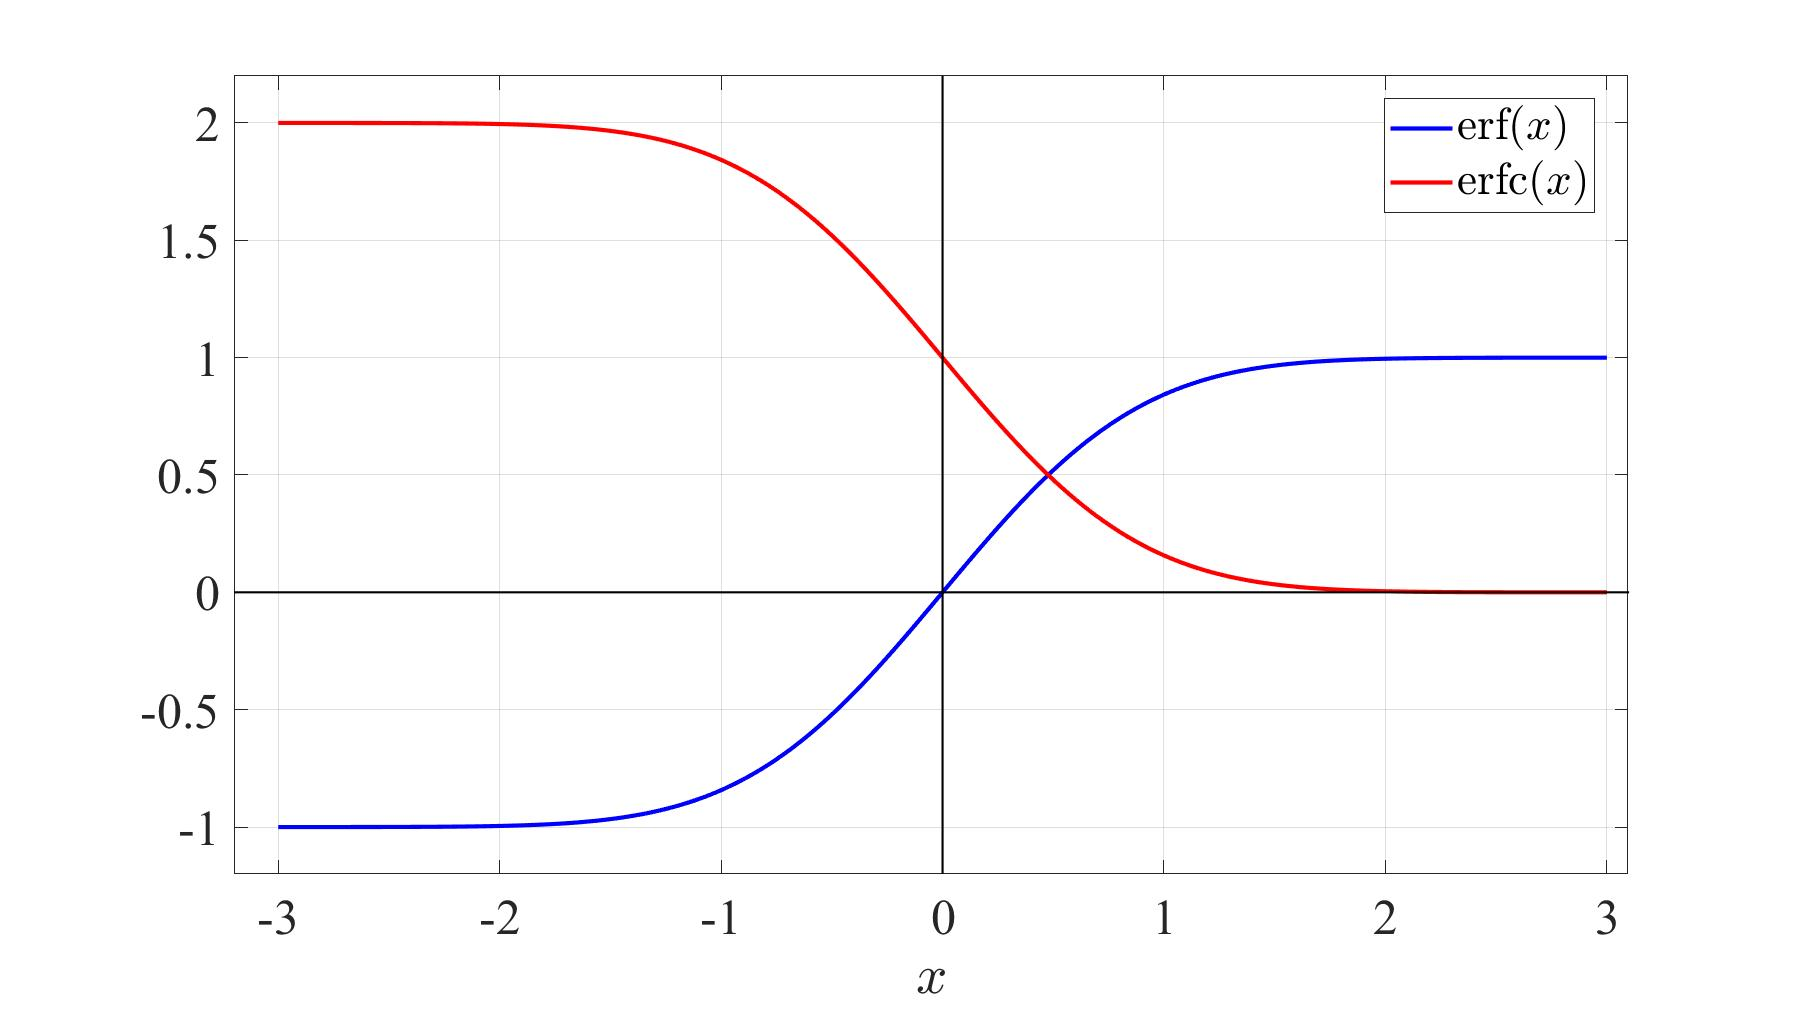
\includegraphics[width=1\textwidth]{matlab/erf.jpg}
	\caption{函数$ \mathrm{erf} \left(x\right)$和$ \mathrm{erfc} \left(x\right)$的图像,其中$-3\le x \le 3$\label{fig:erffig}}
\end{figure}

\begin{property}
	误差函数具有以下的一些基本性质:
	\begin{enumerate}[noitemsep]
		\item $ \mathrm{erf} \left(x\right)$是奇函数,即
		$$ \mathrm{erf} \left(-z\right) =\mathrm{erf} \left(z\right).$$
		这里由于$\displaystyle e^{-t^2}$是偶函数。其极限为
		$$ \lim _{z \rightarrow -\infty} {\mathrm{erf} \left(z\right)} = -1, \lim _{z \rightarrow +\infty} {\mathrm{erf} \left(z\right)} = 1 .$$
		\item 误差函数与误差分布函数的关系为
		$$\mathrm{erf} \left(z\right) + \mathrm{erfc} \left(z\right) =1,\quad \mathrm{erfc}^{-1}\left(1-z\right) = \mathrm{erf}^{-1} \left(z\right).$$
		\item $\mathrm{erf} \left(\overline{z}\right) = \overline{\mathrm{erf} \left( z\right)}.$
		\begin{proof}
			积分函数 $f\left(z\right) = \exp(-z^2)$满足 $$ f(\overline{z})= -\overline{f\left(z\right)}.$$
		\end{proof}
		
	\end{enumerate}
\end{property}

\begin{figure}[ht]
	\centering
	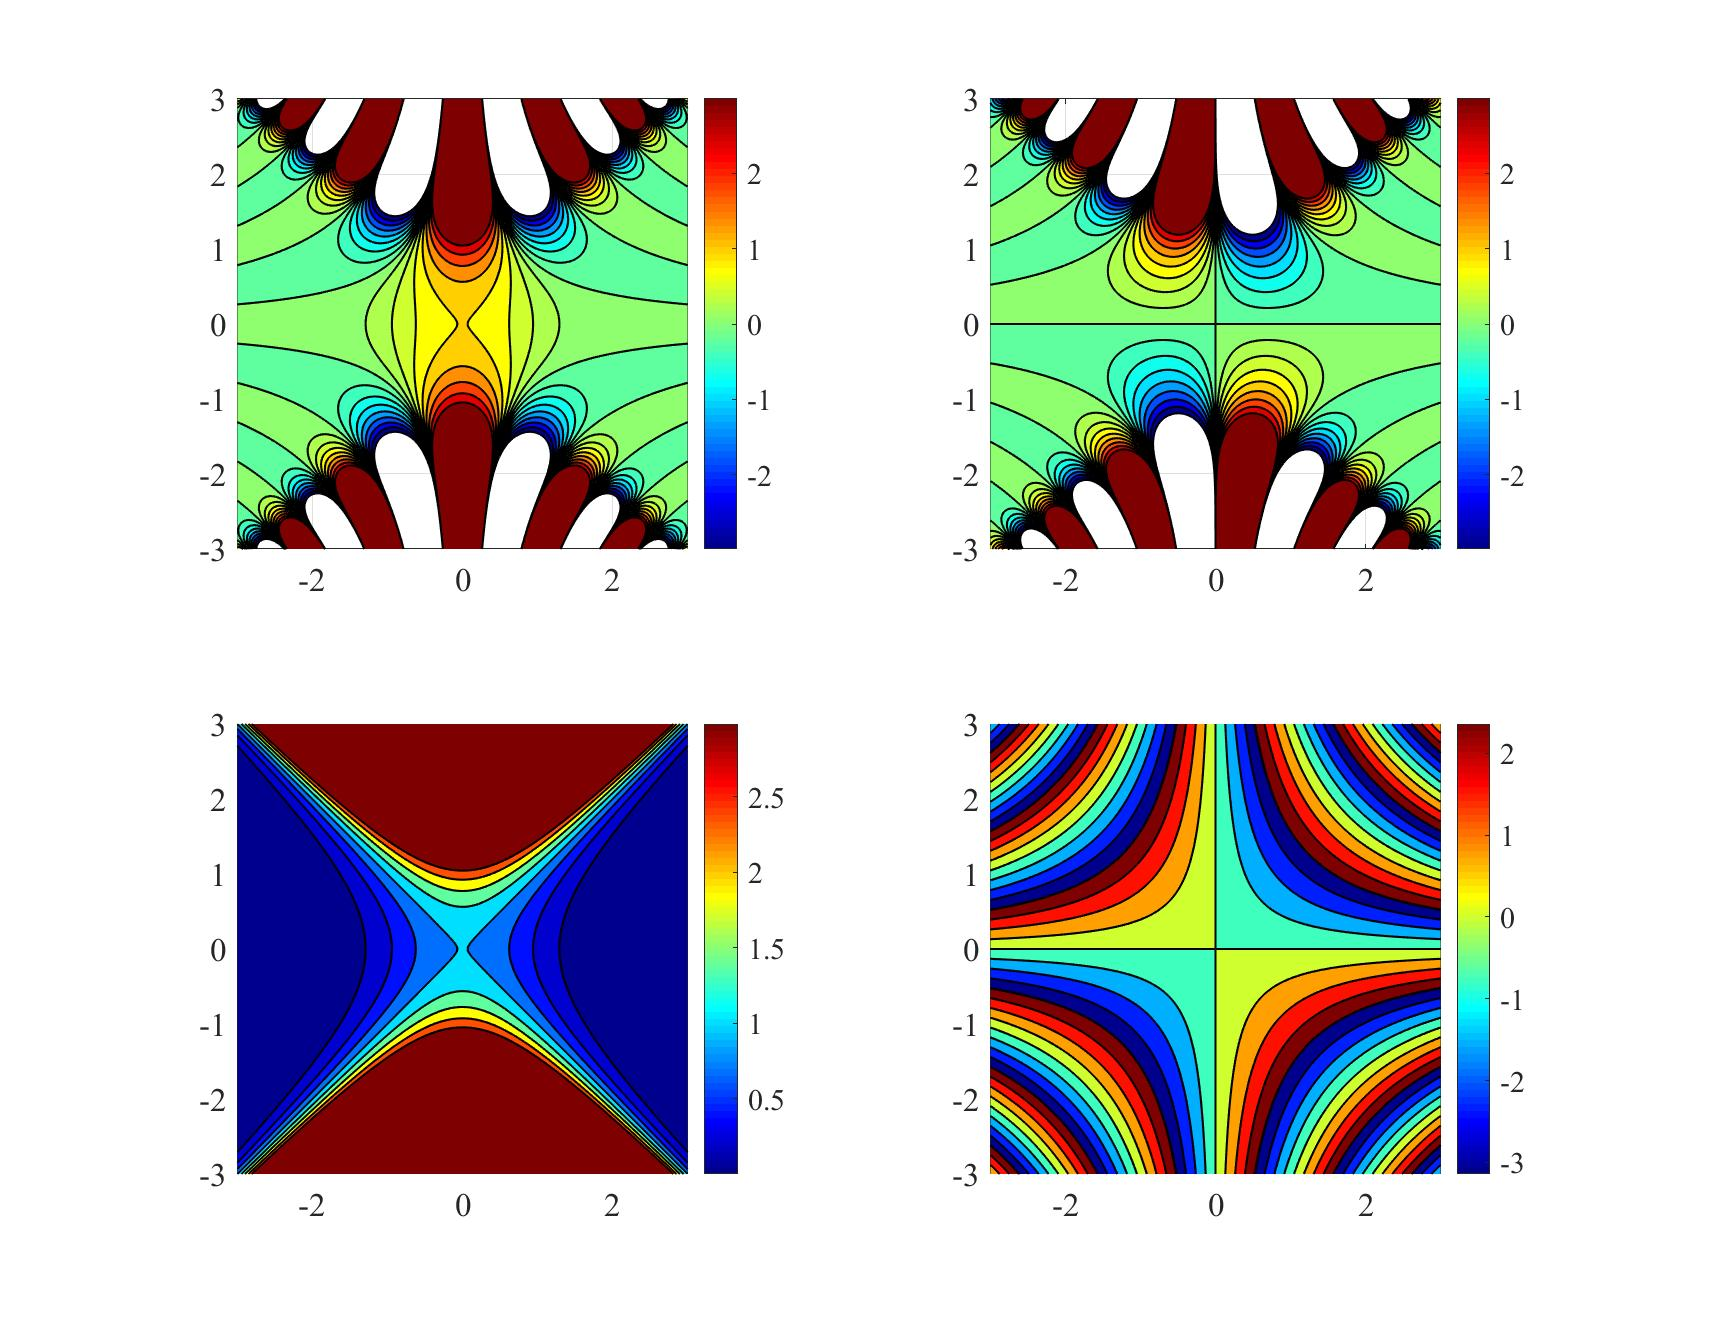
\includegraphics[width=1\textwidth]{matlab/erfz1.jpg}
	\caption{函数$ \mathrm{erf} \left(x\right)$和$ \mathrm{erfc} \left(x\right)$的图像,其中$-3\le x \le 3$\label{fig:erfz1}}
\end{figure}

\begin{figure}[ht]
	\centering
	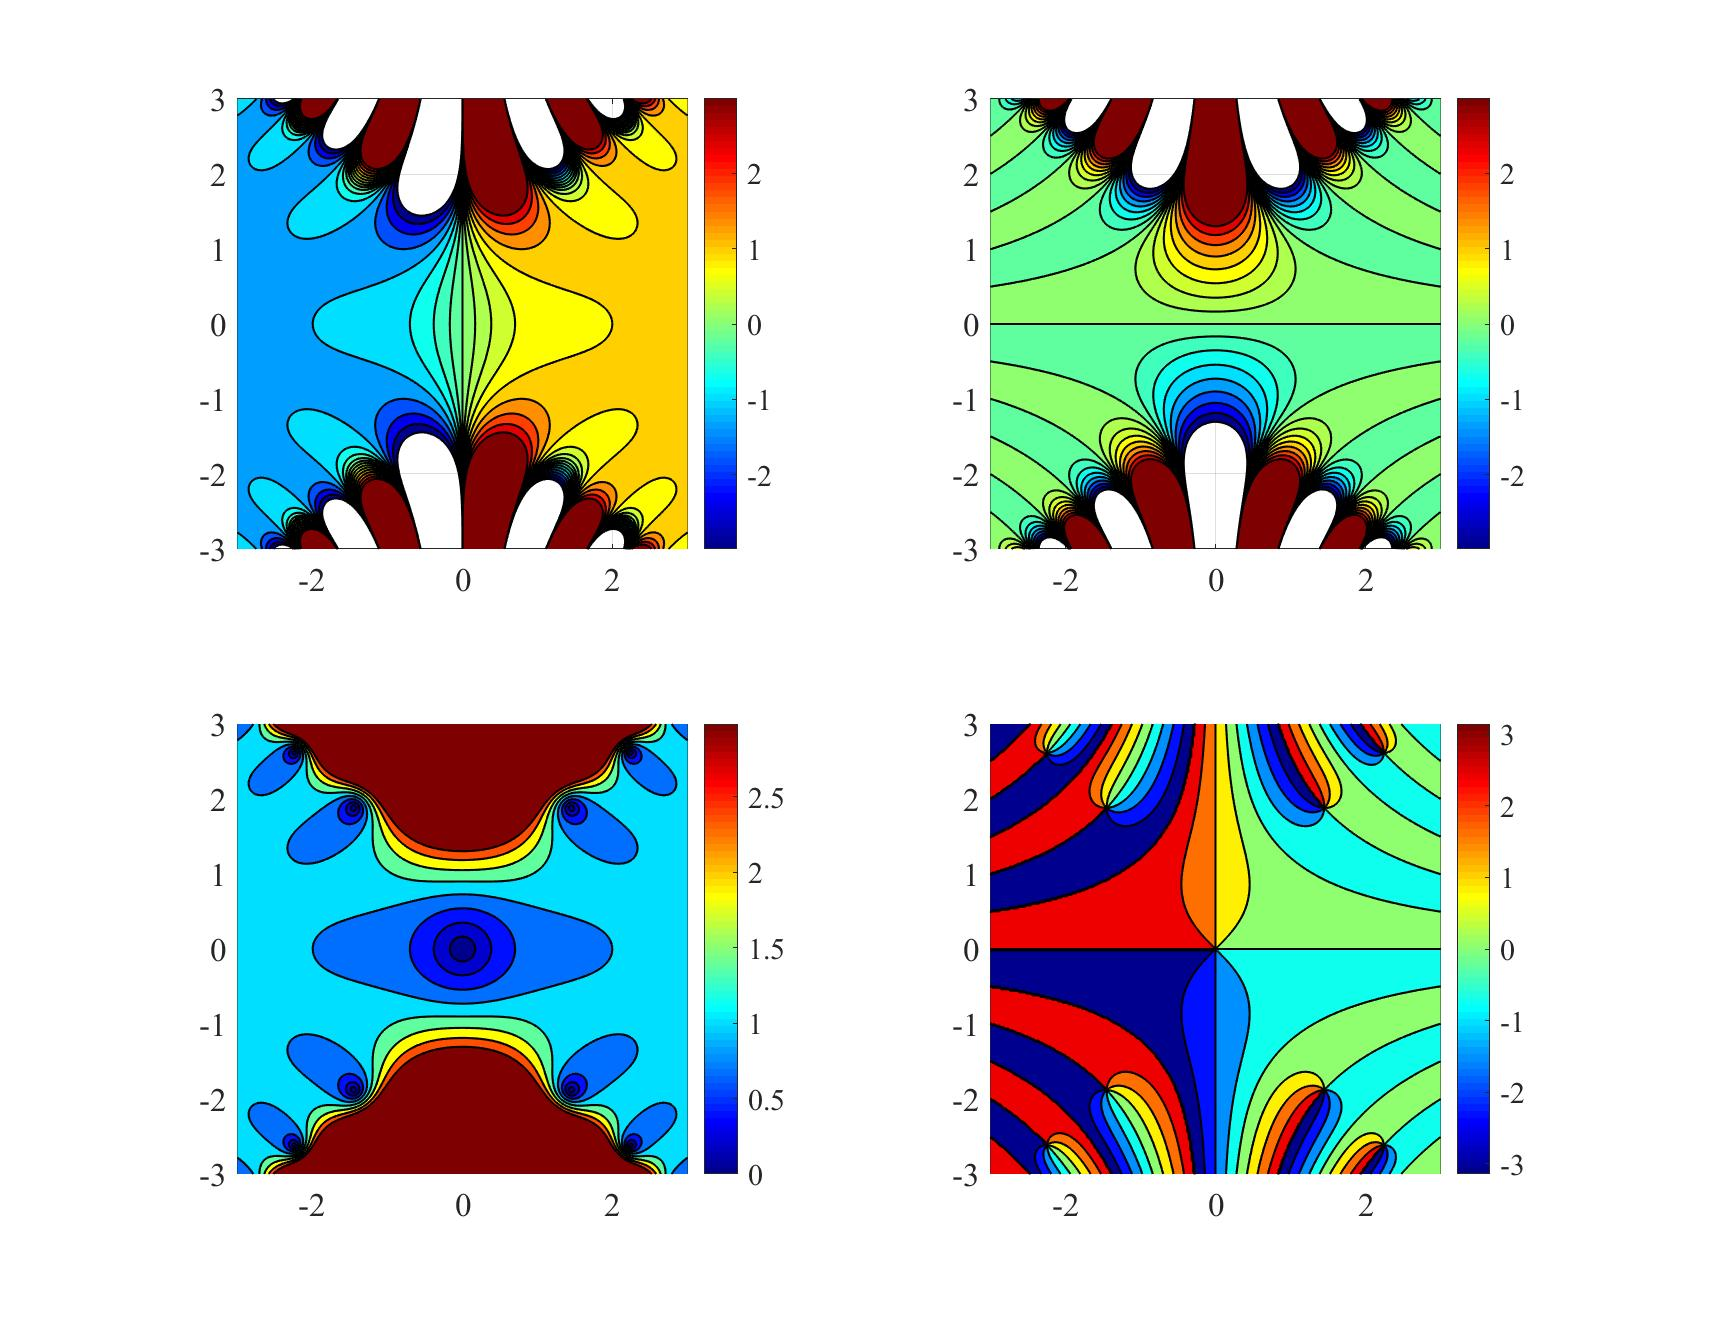
\includegraphics[width=1\textwidth]{matlab/erfz2.jpg}
	\caption{函数$ \mathrm{erf} \left(x\right)$和$ \mathrm{erfc} \left(x\right)$的图像,其中$-3\le x \le 3$\label{fig:erfz2}}
\end{figure}

\subsection{Mittag-Leffler函数}

指数函数$e^x$在整数阶的微分方程中起着非常重要的作用。Mittag-Leffler函数是指数函数的推广,他在分数阶微分方程中起着重要的作用。

\begin{definition}{Mittag-Leffler函数}{Mittag-Leffler Function}
	由级数
	$$E_{\alpha}\left(z\right)=\sum _{k=0}^{+\infty}{\frac{z^k}{\Gamma\left(\alpha k+1\right)}},\quad \alpha>0$$
	定义的函数$E_{\alpha}\left(z\right)$称为单参数Mittag-Leffler函数。更一般,由
	$$E_{\alpha,\beta}\left(z\right)=\sum _{k=0}^{+\infty}{\frac{z^k}{\Gamma\left(\alpha k+\beta\right)}},\quad \alpha>0,\quad \beta>0, $$
	定义的函数$E_{\alpha,\beta}\left(z\right)$称为双参数Mittag-Leffler函数。
\end{definition}

显然有$E_{\alpha,1}\left(z\right) = E_{\alpha}\left(z\right)$,Mittag-Leffler函数满足下面的循环特性,即
\begin{equation}
E_{\alpha,\beta}\left(z\right)=\frac{1}{z} E_{\alpha, \beta-\alpha }\left(z\right)-\frac {1}{z\Gamma\left(\beta -\alpha\right)}.
\end{equation}

\begin{property}
	此外Mittag-Leffler函数具有以下性质:
	\begin{enumerate}[noitemsep]
		\item Mittag-Leffler的积分表示
		\begin{equation}
		E_{{\alpha,\beta }}\left(z\right)={\frac{1}{2\pi i}}\int _{C}{\frac  {t^{{\alpha -\beta }}e^{t}}{t^{\alpha }-z}}\mathrm{d}t.
		\end{equation}
		其中曲线$C$从$-\infty$开始并结束,并围绕被积函数的奇点和分支点旋转。此外有
		\begin{equation}
		\int _{0}^{ +\infty }e^{-t}t^{\beta -1}E_{\alpha ,\beta }\left(t^{\alpha} z\right)\mathrm{d}t={\frac{1}{1-z}}.
		\end{equation}
		\item Laplace积分变换
		函数$t^{\beta -1}E_{\alpha ,\beta }\left(t^{\alpha }\right)$和$t^{\beta -1}E_{\alpha ,\beta }\left(-t^{\alpha }\right)$的Laplace变换为
		
		\begin{equation}
		\int _{0}^{\infty }e^{-pt}t^{\beta -1}E_{\alpha ,\beta }\left(t^{\alpha }\right)\mathrm{d}t={\frac {p^{\alpha-\beta }}{p^{\alpha}-1}}={\frac {p^{-\beta }}{1-p^{-\alpha}}}, \qquad \mathrm{Re}\left(p\right)>1.
		\end{equation}
		
		\begin{equation}
		\int _{0}^{\infty }e^{-pt}t^{\beta -1}E_{\alpha ,\beta }\left(-t^{\alpha }\right)\mathrm{d}t={\frac {p^{\alpha-\beta }}{1+p^{\alpha}}}={\frac {p^{-\beta }}{1+p^{-\alpha}}}, \qquad \mathrm{Re}\left(p\right)>1.
		\end{equation}
		
		特别的当$\beta = 1$可以得到Mittag-Leffler函数的Laplace变换。
		\begin{equation}
		\int _{0}^{\infty }e^{-pt}E_{\alpha}\left(t^{\alpha }\right)\mathrm{d}t={\frac {p^{\alpha-1}}{p^{\alpha}-1}}={\frac {1}{p-p^{1-\alpha}}}, \qquad \mathrm{Re}\left(p\right)>1.
		\end{equation}
		
		\begin{equation}
		\int _{0}^{\infty }e^{-pt}E_{\alpha}\left(-t^{\alpha }\right)\mathrm{d}t={\frac {p^{\alpha-1}}{1+p^{\alpha}}}={\frac {1}{p+p^{1-\alpha}}}, \qquad \mathrm{Re}\left(p\right)>1.
		\end{equation}
		
		\begin{table}[htbp]
			\centering\makegapedcells
			\caption{某些特殊的Mittag-Leffler函数}
			\setlength{\tabcolsep}{7mm}
			\label{tab:Table2-1-1}
			\begin{tabular}{l*{4}{c}}
				\toprule
				$ \alpha$  & $ \displaystyle E_{\alpha,1}\left(z\right)$  & $ \displaystyle f\left(z\right)$   & $ \displaystyle \int_{0}^{z}{E_{\alpha,1}\left(-s^2\right)} {\mathrm{d}s}$ \\
				\midrule
				$\displaystyle 0$   & $ \displaystyle \sum _{{k=0}}^{+\infty }z^{k}  $  & $\displaystyle \frac{1}{1-z}$       & $ \arctan\left(z\right)$ \\
				$ \displaystyle \frac{1}{2}$ & $\displaystyle \sum _{k=0}^{+\infty }{\frac{z^{k}}{\Gamma\left(k+\frac{1}{2}\right)}}$  & $\displaystyle e^{z^2} \mathrm{erfc}\left(-z\right)$ &   \\   	
				$\displaystyle 1$   & $\displaystyle \sum _{k=0}^{+\infty }{\frac{z^{k}}{\Gamma\left(k+1\right)}}$   & $\displaystyle e^{z}$  & $ \displaystyle \frac{\sqrt{\pi}}{2}\mathrm{erf}\left(z\right)$  \\    
				$2$    & $\displaystyle \sum _{k=0}^{+\infty }{\frac{z^{k}}{\Gamma\left(k+2\right)}}$    & $ \displaystyle \cosh\left(\sqrt{z}\right) $ & $\displaystyle {\sin}\left(z\right)$     \\
				\bottomrule
			\end{tabular}
		\end{table}
		
		此外,对于$\beta = 1$时,Mittag-Leffler函数可以表示某些特殊的函数,如\tabref{tab:Table2-1-1}所示。
		
	\end{enumerate}
\end{property}

\section{Riemann-Liouville分数阶积分和分数阶导数}

Abel方程是一个积分方程  \hint{【参考文献】}
\begin{equation}
\frac{1}{\Gamma\left(\alpha\right)} \int_{a}^{x} \frac{\phi\left(t\right)\mathrm{d}t}{\left(x-t\right)^{1-\alpha}}=f\left(x\right),\quad x>a,\quad 0<a<1.
\end{equation}

此方程的求解可以按照下述方法进行求解:方程两边同事乘以$\left(x-t\right)^{-\alpha}$,并从$a$到$x$进行积分,得到







